\subsection{Trained answers without instructions}
\label{sec:nodeftrained}

This subsection puts the recogniser in front of trained adapters and compares it with the two published methods of Section~\ref{sec:nodefpublished}, first on a small model and then on the model of the main runs. It uses the routes tested in Section~\ref{sec:recogniser}. The lines for each run were again fixed before it.

\paragraph{Trained answers on a small model.} The stand-alone code (\texttt{t5-small}, the five tasks, no definition in any input, one seed, on a CPU; first used for an earlier pilot reported in Section~\ref{sec:noinstruction}) was run with the routes of \recog{} on the frozen states of that small model, by the lines of that pilot: at most 20 of 200 answers changed and forgetting at most 3 points while more than 100 change with all adapters on; the score right after learning at least 90\% of that with all adapters on; at least 80\% of the test inputs at their own task.
With all adapters on, \AudSmallAllChanged{} of \AudSmallAllCompared{} answers to earlier tasks changed and the score fell from \AudSmallAllLearned{} to \AudSmallAllAP{}; with the routes, \AudSmallRidgeChanged{} of \AudSmallRidgeCompared{} changed, forgetting was \AudSmallRidgeFT{}, the score went from \AudSmallRidgeLearned{} to \AudSmallRidgeAP{}, and 97.2\% of the test inputs reached their own task: ``works''.
Two of the five tasks are learned poorly by this small model under either rule, so they add little to the comparison. This check was planned before the GPU run of the next paragraph and finished after it.

\paragraph{Trained answers: our method against the published methods, without instructions.} The same five-task run as in Section~\ref{sec:nodefpublished}, on a GPU, with plain adapters that are never blocked: while task $t$ is learned, adapters $1$ to $t$ are on for all its inputs, and at test time an input is answered by the adapters that existed when the task it is routed to was learned.
The routes of \recog{} and \handicap{} ($\nu = 2$), on the frozen T5-base states of the instance, were written to the repository before the run (Table~\ref{tab:routesgpu}, at the end of this subsection).
Line fixed before the run: ``beats the published methods in this setting'' if all three hold: the final score is at least 2 points above the better published method without definitions; forgetting is below 2 points; at most 32 of the \AudOursRidgeCompared{} compared answers change (a quarter of what GainLoRA changes).
``Does not'' if the final score is below that of the better published method or at least \AudPubGainloraNoDefChanged{} answers change; anything else is ``mixed''.
For \recog{} the final score is \AudOursRidgeAP{} against \AudPubGainloraNoDefAP{} for GainLoRA, forgetting is \AudOursRidgeFT{}, and \AudOursRidgeChanged{} of \AudOursRidgeCompared{} answers changed.
For \handicap{} the figures are \AudOursHandicapAP{}, \AudOursHandicapFT{} and \AudOursHandicapChanged{} of \AudOursHandicapCompared{}.
All three lines hold for both, so the verdict is ``beats the published methods in this setting''.
Our guesses for \recog{}, 5 to 15 changed answers and forgetting below 1 point, held; they were written before \handicap{} was added to the table.
Five things must be said with it.

(a) The line said ``official test'', but the official test scores the plain adapters with all of them on (final score \AudOffOursNoDefAP{}); the routed rules exist only in the re-test.
So the re-test is compared with the re-test.
The two scorings of the published methods differ little (\AudPubGainloraNoDefAP{} against \AudOffGainloraNoDefAP{} for GainLoRA, \AudPubInfloraNoDefAP{} against \AudOffInfloraNoDefAP{} for InfLoRA).

(b) At 10 epochs most of the gap in the final score is learning, not retention.
Our guess for the score right after learning was 54 to 58, because we assumed that our adapters would learn as poorly without definitions as the published methods do; it was far too low: it is \AudOursRidgeLearned{}.
Plain adapters learn the five tasks almost as well without the definitions (\AudOursAllLearned{}) as with them (\AudWordOriginalAllLearned{}), with sst2 at \AudOursPtLearnedSst{} and emotion at \AudOursPtLearnedEmotion{}, where the published methods reach \AudPubInfloraNoDefPtLearnedSst{} and \AudPubGainloraNoDefPtLearnedSst{} on sst2 and \AudPubInfloraNoDefPtLearnedEmotion{} and \AudPubGainloraNoDefPtLearnedEmotion{} on emotion (Table~\ref{tab:noinstpertask} in Section~\ref{sec:nodefpublished}).
These two methods restrict what a new adapter may change, to protect the old tasks, and with a tenth of their published number of epochs they learn two of the five tasks poorly; with their full number of epochs they learn them (the paragraph on \AudFullEpochs{} epochs below).
The columns that are about retention are forgetting and changed answers: \AudOursRidgeFT{} and \AudOursHandicapFT{} for ours against \AudPubGainloraNoDefFT{} and \AudPubInfloraNoDefFT{} for the published methods, and \AudOursRidgeChanged{} and \AudOursHandicapChanged{} changed answers against \AudPubGainloraNoDefChanged{} and \AudPubInfloraNoDefChanged{}.
These are less tied to learning than the final score, but not free of it: forgetting cannot exceed what was learned, and the answers of a method that has learned less may be less stable. The run of the published methods at their published number of epochs, below, separates the two.

(c) Our final score without any definition is also above the published methods with their definitions (\AudPubGainloraDefAP{} for GainLoRA and \AudPubInfloraDefAP{} for InfLoRA), with the same caveat on learning. We had expected GainLoRA with definitions to stay ahead of ours without them; it did not.

(d) The audit next to what happened (Table~\ref{tab:routesgpu}): over the first four tasks the audit of \recog{} says \AudRouteFiveRidgeFirstFourAuditEst{}\% of the routes changed on average, with 95\% bounds per task from \AudRouteFiveRidgeFirstFourBoundLow{}\% to \AudRouteFiveRidgeFirstFourBoundHigh{}\%; \AudRouteFiveRidgeChanged{} of their \AudRouteFiveRidgeCompared{} routes changed (\AudRouteFiveRidgeChangedShare{}\%). Each changed route changed its answer, and no other answer changed.
For \handicap{} it is \AudRouteFiveHandicapChanged{} of \AudRouteFiveHandicapCompared{}; the audit is not valid for it on the same held-out inputs (Remark~\ref{rem:auditlimits}(iii)).

(e) It is one sequence of five tasks and a small model: a first sign and no more. The published methods were run with their full number of epochs for one seed only (below). The five tasks are among the 15 on which the rule and its one setting were chosen, and that choice looked at the test inputs of those tasks; the choice was between variants that differ by at most 1.5 points there (Table~\ref{tab:recogniserdev} in Section~\ref{sec:recogniser}), but the routes of this run are in that sense development routes, and only the fresh batches test the recogniser on tasks it was not chosen on.

\paragraph{Three seeds.} After the first seed had been read, seeds 43 and 44 were run for the published methods and for ours (the route table does not depend on the seed; only the adapters differ).
Reading fixed before these runs: the verdict stands for three seeds if the three lines hold for the means over the seeds and the final score of \recog{} is above that of the better published method in every single seed.
Table~\ref{tab:noinstseeds} gives the means.
The final score of \recog{} is \AudSeedsRidgeAP{} (\AudSeedsRidgeAPLow{} to \AudSeedsRidgeAPHigh{} over the seeds) against \AudSeedsGainloraAP{} for GainLoRA and \AudSeedsInfloraAP{} for InfLoRA; its forgetting is \AudSeedsRidgeFT{} points, and \AudSeedsRidgeChanged{} of \AudSeedsCompared{} answers changed, against \AudSeedsGainloraChanged{} and \AudSeedsInfloraChanged{}.
\handicap{} ends at \AudSeedsHandicapAP{} with \AudSeedsHandicapChanged{} changed answers.
\recog{} is above the better published method in \AudSeedsRidgeAboveInAll{} of \AudSeedsN{} seeds, so the verdict stands for three seeds, with the same five things to be said.
Our guesses for these seeds (a final score of 76 to 79 in each, 4 to 9 changed answers of 400 for \recog{} and 0 to 3 for \handicap{}) held.
Our three seeds differ little, as expected, since the routes are the same in every seed.
The simpler rule \centre{} (the nearest centre of word-vectors of the whole input, Section~\ref{sec:method}) ends at \AudSeedsCentreAP{} with \AudSeedsCentreChanged{} changed answers: even this simple rule goes most of the way here; \recog{} and \handicap{} add about three points (the ceiling is \AudSeedsOwnAP{}), fewer changed answers, and the audit and the bound.

\paragraph{The published methods with their published number of epochs.} Point (b) left open whether the two published methods close the gap with their full training. So both were run once more without definitions with \AudFullEpochs{} epochs per task, the published number, on the same five tasks (seed 42, T5-base; Table~\ref{tab:noinstfull}).
Lines fixed before the run: ``they close the learning gap'' if the score right after learning reaches at least 73, within five points of ours with 10 epochs, and ``they do not'' below 65; ``they hold their answers less well than ours'' if forgetting is at least 5 points above ours or at least 60 more of the \AudFullCompared{} answers change than under \recog{}, and ``no such sign'' if forgetting is within 2 points of ours and at most 25 more answers change.
Both lines are met.
With \AudFullEpochs{} epochs the two methods learn the five tasks as well as plain adapters do with 10 (\AudFullInfloraLearned{} for InfLoRA and \AudFullGainloraLearned{} for GainLoRA right after learning, against \AudOursRidgeLearned{}), and a little less than plain adapters with \AudFullEpochs{} epochs (\AudFullOursRidgeLearned{}). They now learn sst2 and emotion, the two tasks they had learned poorly (Table~\ref{tab:noinstfullpertask}).
Then they lose them: forgetting is \AudFullInfloraFT{} and \AudFullGainloraFT{} points, \AudFullInfloraChanged{} and \AudFullGainloraChanged{} of \AudFullCompared{} answers change, and the final scores are \AudFullInfloraAP{} and \AudFullGainloraAP{}, against \AudOursRidgeAP{} for plain adapters behind \recog{} with a tenth of the epochs (\AudOursRidgeFT{} points of forgetting, \AudOursRidgeChanged{} changed answers) and \AudFullOursRidgeAP{} with the same number of epochs (next paragraph).
From 10 to \AudFullEpochs{} epochs their forgetting grew with what they had learned: from \AudPubInfloraNoDefFT{} to \AudFullInfloraFT{} points for InfLoRA and from \AudPubGainloraNoDefFT{} to \AudFullGainloraFT{} for GainLoRA.
So in this run the gap in the final score is forgetting and not learning; the first sentence of point (b) belongs to the comparison at 10 epochs.
Our guesses were partly wrong, and wrong in the direction of too little forgetting: we had expected them to learn 68 to 78 (right; InfLoRA is just above), to change 60 to 200 answers (right for GainLoRA, far too few for InfLoRA) and to forget 4 to 15 points (wrong for both).
One limit belongs to this run: it is one seed and five tasks on T5-base, where the published setting uses a larger model. Why the two methods lose their answers is the question of the control below.

\paragraph{Our rules with the same number of epochs.} The comparison above gives the published methods ten times the training of ours. So plain adapters were also trained for \AudFullEpochs{} epochs per task (seed 42, no definitions, the same route table; top of Table~\ref{tab:noinstfull}).
Line fixed before the run: ``beats the published methods at equal epochs, in this setting'' if the final score of \recog{} is at least 2 points above the better published method at \AudFullEpochs{} epochs, forgetting is below 2 points, and at most 44 of \AudFullCompared{} answers change (a quarter of what GainLoRA changes); ``does not'' if the final score is below that method's.
All three hold. \recog{} ends at \AudFullOursRidgeAP{}, \AudFullOursRidgeAboveGainlora{} points above GainLoRA, with \AudFullOursRidgeFT{} points of forgetting and \AudFullOursRidgeChanged{} changed answers; \handicap{} ends at \AudFullOursHandicapAP{} with \AudFullOursHandicapChanged{}.
Right after learning the three ways are close (\AudFullOursRidgeLearned{} for ours, \AudFullInfloraLearned{} and \AudFullGainloraLearned{} for the published methods), so at equal training the gap in the final score is retention.
Lemma~\ref{lem:route} said in advance that at most as many answers can change as routes: the routes do not depend on the adapters, so they are the routes of the 10-epoch run; here exactly as many answers changed as routes, \AudFullOursRidgeChanged{} under \recog{} and \AudFullOursHandicapChanged{} under \handicap{}. Ten times the training changed no further answer.
The forgetting of \recog{} is \AudFullOursRidgeFT{} points here against \AudOursRidgeFT{} with 10 epochs: the same inputs go to another task, and a wrong route costs more when the adapters are better.
Our guesses held (a score right after learning of 77 to 82, a final score within one point of it, 3 to 6 changed answers); our doubt that more epochs might not help plain adapters was wrong, the score right after learning rose by \AudFullOursLearnedGain{} points.
It is one seed and five tasks. Figure~\ref{fig:answergrid} shows the changed answers one by one, and Figure~\ref{fig:stageheat} the score of every task after every stage.

\begin{figure}[t]
  \centering
  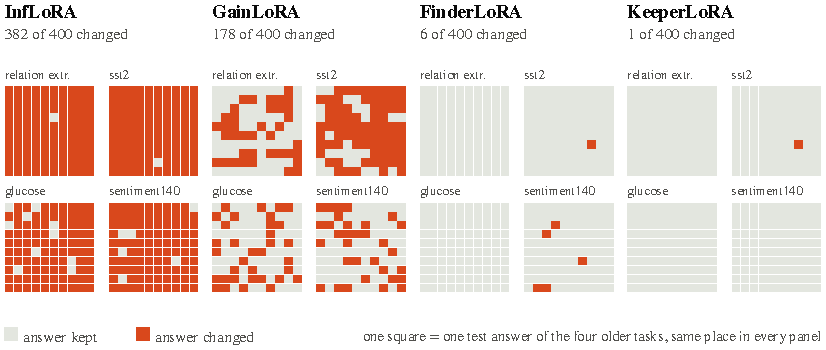
\includegraphics[width=\linewidth]{figures/answer_grid}
  \caption{Every square is one test answer. Five tasks without definitions, \AudFullEpochs{}
  epochs per task, seed 42: the \AudFullCompared{} test answers of the four older tasks, right
  after their task was learned against after the last task; a square has the same place in every
  panel. InfLoRA changes \AudFullInfloraChanged{} of the \AudFullCompared{} answers, GainLoRA
  \AudFullGainloraChanged{}, \recog{} \AudFullOursRidgeChanged{} and \handicap{}
  \AudFullOursHandicapChanged{}.}
  \label{fig:answergrid}
\end{figure}

\begin{figure}[t]
  \centering
  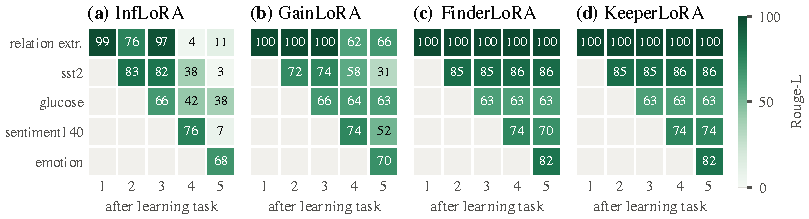
\includegraphics[width=\linewidth]{figures/stage_heatmap}
  \caption{The score of each task (rows) after each later task has been learned (columns), for the
  runs of Figure~\ref{fig:answergrid}; Rouge-L of the re-test (all reference answers), rounded. A
  row that keeps its colour is a task that is not forgotten: with InfLoRA and GainLoRA most rows of
  older tasks fade, with \recog{} and \handicap{} they stay.}
  \label{fig:stageheat}
\end{figure}


\paragraph{The control: the same methods with their definitions.} The run above cannot say by itself why the published methods lose their answers: the loss could come from the missing definition, or from \AudFullEpochs{} epochs on this smaller model. So the two methods were run once more with \AudFullEpochs{} epochs and the definitions left in; the seed, the tasks, the model and the code are the same, and the definition in the input is the only difference (Table~\ref{tab:fulldefinitions}).
Line fixed before the run, for each method: ``the instruction was what kept the answers'' if, with definitions, forgetting is at most half of its value without them and at most half as many answers change; ``it was not the instruction'' if forgetting with definitions is at least 80\% of that without.
The first holds for both. With definitions GainLoRA forgets \AudFullDefOriginalGainloraFT{} points and changes \AudFullDefOriginalGainloraChanged{} of \AudFullDefCompared{} answers, against \AudFullGainloraFT{} points and \AudFullGainloraChanged{} answers without; InfLoRA forgets \AudFullDefOriginalInfloraFT{} points and changes \AudFullDefOriginalInfloraChanged{} answers, against \AudFullInfloraFT{} and \AudFullInfloraChanged{}. The two differ in size: with their definitions GainLoRA holds nearly all its answers, InfLoRA fewer, so the instruction is what held most of their answers.
\recog{} and \handicap{}, which never read the definition, forget \AudFullOursRidgeFT{} and \AudFullOursHandicapFT{} points without it.
Two more things were to be reported as they are.
With their definitions and \AudFullEpochs{} epochs the two methods end at \AudFullDefOriginalInfloraAP{} (InfLoRA) and \AudFullDefOriginalGainloraAP{} (GainLoRA), below \cert{} and \recog{} with definitions and 10 epochs (\AudUOriginalCertAP{} and \AudUOriginalRidgeAP{}, Section~\ref{sec:exampleroutes}); we did not train our adapters for \AudFullEpochs{} epochs with definitions.
Under the heavy rewording they end at \AudFullDefHeavyInfloraAP{} and \AudFullDefHeavyGainloraAP{} with \AudFullDefHeavyInfloraChanged{} and \AudFullDefHeavyGainloraChanged{} changed answers (Table~\ref{tab:fullwordings}).
Our guesses were right for InfLoRA and for the forgetting of GainLoRA; GainLoRA learned less than we had guessed (\AudFullDefOriginalGainloraLearned{} right after learning, where we had said 79 to 84), and we had thought it more likely than not that it would end above our 10-epoch score, which it did not.
It is one seed and five tasks on T5-base. Figure~\ref{fig:learnkeep} puts the runs with and without definitions side by side.

\begin{figure}[t]
  \centering
  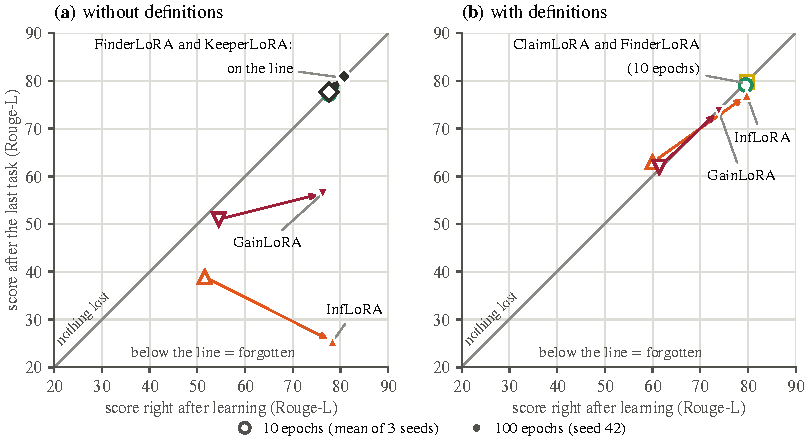
\includegraphics[width=\linewidth]{figures/learn_keep}
  \caption{Learned against kept, five tasks. A point is a method: its mean score right after
  learning ($x$) and after the last task ($y$). On the diagonal nothing is lost; the distance below
  it is what was forgotten. Hollow: 10 epochs (mean of three seeds); filled: \AudFullEpochs{} epochs
  (seed 42); an arrow goes from 10 to \AudFullEpochs{} epochs. (a)~Without definitions the two
  published methods learn more with more epochs and fall further below the diagonal; \recog{} and
  \handicap{} stay on it. (b)~With definitions the published methods stay near the diagonal (the
  control run); for our rules with definitions only 10-epoch runs exist.}
  \label{fig:learnkeep}
\end{figure}


\begin{table}[t]
  \caption{The definition as the only difference: the two published methods with \AudFullEpochs{} epochs per task, with their definitions and without them (five tasks, seed 42, T5-base, re-test), and \recog{} and \handicap{} without definitions at the same number of epochs.}
  \label{tab:fulldefinitions}
  \centering
  {\footnotesize\setlength{\tabcolsep}{3pt}\begin{tabular}{p{1.9in}lrrrr}
    \toprule
    Method (seed 42, 100 epochs) & Definitions & \shortstack[r]{Score right\\after\\learning $\uparrow$} & \shortstack[r]{Final\\score $\uparrow$} & \shortstack[r]{Forgetting\\(points) $\downarrow$} & \shortstack[r]{Answers\\changed\\of \AudFullDefCompared{} $\downarrow$} \\
    \midrule
    InfLoRA & with & \AudFullDefOriginalInfloraLearned{} & \AudFullDefOriginalInfloraAP{} & \AudFullDefOriginalInfloraFT{} & \AudFullDefOriginalInfloraChanged{} \\
    InfLoRA & none & \AudFullInfloraLearned{} & \AudFullInfloraAP{} & \AudFullInfloraFT{} & \AudFullInfloraChanged{} \\
    \midrule
    GainLoRA & with & \AudFullDefOriginalGainloraLearned{} & \AudFullDefOriginalGainloraAP{} & \AudFullDefOriginalGainloraFT{} & \AudFullDefOriginalGainloraChanged{} \\
    GainLoRA & none & \AudFullGainloraLearned{} & \AudFullGainloraAP{} & \AudFullGainloraFT{} & \AudFullGainloraChanged{} \\
    \midrule
    \recog{} (ours) & none & \AudFullOursRidgeLearned{} & \AudFullOursRidgeAP{} & \AudFullOursRidgeFT{} & \AudFullOursRidgeChanged{} \\
    \handicap{} (ours) & none & \AudFullOursHandicapLearned{} & \AudFullOursHandicapAP{} & \AudFullOursHandicapFT{} & \AudFullOursHandicapChanged{} \\
    \bottomrule
\end{tabular}}

\end{table}

\begin{table}[t]
  \caption{The two published methods with their definitions and \AudFullEpochs{} epochs per task under the four wordings of the definition (seed 42, re-test); below, for reference, \cert{} and \recog{} with definitions and 10 epochs (Table~\ref{tab:instanceroutes}).}
  \label{tab:fullwordings}
  \centering
  {\scriptsize\setlength{\tabcolsep}{2pt}\begin{tabular}{p{1.2in}rrrrrrrr}
    \toprule
    & \multicolumn{4}{c}{Final score $\uparrow$} & \multicolumn{4}{c}{\shortstack{Answers changed\\of \AudFullDefCompared{} $\downarrow$}} \\
    \cmidrule(lr){2-5}\cmidrule(l){6-9}
    & original & light & medium & heavy & original & light & medium & heavy \\
    \midrule
    InfLoRA, 100 epochs & \AudFullDefOriginalInfloraAP{} & \AudFullDefLightInfloraAP{} & \AudFullDefMediumInfloraAP{} & \AudFullDefHeavyInfloraAP{} & \AudFullDefOriginalInfloraChanged{} & \AudFullDefLightInfloraChanged{} & \AudFullDefMediumInfloraChanged{} & \AudFullDefHeavyInfloraChanged{} \\
    GainLoRA, 100 epochs & \AudFullDefOriginalGainloraAP{} & \AudFullDefLightGainloraAP{} & \AudFullDefMediumGainloraAP{} & \AudFullDefHeavyGainloraAP{} & \AudFullDefOriginalGainloraChanged{} & \AudFullDefLightGainloraChanged{} & \AudFullDefMediumGainloraChanged{} & \AudFullDefHeavyGainloraChanged{} \\
    \midrule
    \cert{}, 10 epochs & \AudUOriginalCertAP{} & \AudULightCertAP{} & \AudUMediumCertAP{} & \AudUHeavyCertAP{} & \AudUOriginalCertChanged{} & \AudULightCertChanged{} & \AudUMediumCertChanged{} & \AudUHeavyCertChanged{} \\
    \recog{}, 10 epochs & \AudUOriginalRidgeAP{} & \AudULightRidgeAP{} & \AudUMediumRidgeAP{} & \AudUHeavyRidgeAP{} & \AudUOriginalRidgeChanged{} & \AudULightRidgeChanged{} & \AudUMediumRidgeChanged{} & \AudUHeavyRidgeChanged{} \\
    \bottomrule
\end{tabular}}

\end{table}

\begin{table}[t]
  \caption{The five tasks without definitions, seed 42, T5-base, re-test: plain adapters behind \recog{} and \handicap{} and the two published methods, each with \AudFullEpochs{} epochs per task (the published number) and with 10. Score right after learning: average score right after each task was learned; Final score: average final score; Answers changed: answers to the test inputs of the first four tasks that differ at the end from the answer right after their task was learned.}
  \label{tab:noinstfull}
  \centering
  {\footnotesize\setlength{\tabcolsep}{3pt}\begin{tabular}{p{1.95in}rrrr}
    \toprule
    Method, epochs (seed 42, no definition) & \shortstack[r]{Score right\\after\\learning $\uparrow$} & \shortstack[r]{Final\\score $\uparrow$} & \shortstack[r]{Forgetting\\(points) $\downarrow$} & \shortstack[r]{Answers\\changed\\of \AudFullCompared{} $\downarrow$} \\
    \midrule
    \recog{} (ours), 100 epochs & \AudFullOursRidgeLearned{} & \AudFullOursRidgeAP{} & \AudFullOursRidgeFT{} & \AudFullOursRidgeChanged{} \\
    \handicap{} (ours), 100 epochs & \AudFullOursHandicapLearned{} & \AudFullOursHandicapAP{} & \AudFullOursHandicapFT{} & \AudFullOursHandicapChanged{} \\
    \midrule
    InfLoRA, 100 epochs & \AudFullInfloraLearned{} & \AudFullInfloraAP{} & \AudFullInfloraFT{} & \AudFullInfloraChanged{} \\
    GainLoRA, 100 epochs & \AudFullGainloraLearned{} & \AudFullGainloraAP{} & \AudFullGainloraFT{} & \AudFullGainloraChanged{} \\
    \midrule
    InfLoRA, 10 epochs & \AudPubInfloraNoDefLearned{} & \AudPubInfloraNoDefAP{} & \AudPubInfloraNoDefFT{} & \AudPubInfloraNoDefChanged{} \\
    GainLoRA, 10 epochs & \AudPubGainloraNoDefLearned{} & \AudPubGainloraNoDefAP{} & \AudPubGainloraNoDefFT{} & \AudPubGainloraNoDefChanged{} \\
    \midrule
    \recog{} (ours), 10 epochs & \AudOursRidgeLearned{} & \AudOursRidgeAP{} & \AudOursRidgeFT{} & \AudOursRidgeChanged{} \\
    \handicap{} (ours), 10 epochs & \AudOursHandicapLearned{} & \AudOursHandicapAP{} & \AudOursHandicapFT{} & \AudOursHandicapChanged{} \\
    \bottomrule
\end{tabular}}

\end{table}

\begin{table}[t]
  \caption{The two published methods without definitions with \AudFullEpochs{} epochs per task, seed 42, official test (one random reference answer): score of each task right after it was learned and after the last task.}
  \label{tab:noinstfullpertask}
  \centering
  {\footnotesize\setlength{\tabcolsep}{2pt}\begin{tabular}{lrr}
    \toprule
    & \multicolumn{2}{c}{\shortstack{Score right after\\learning $\to$ at the end $\uparrow$}} \\
    \cmidrule(l){2-3}
    Task & InfLoRA & GainLoRA \\
    \midrule
    relation extr. & \AudFullInfloraPtLearnedRelation{}\,$\to$\,\AudFullInfloraPtFinalRelation{} & \AudFullGainloraPtLearnedRelation{}\,$\to$\,\AudFullGainloraPtFinalRelation{} \\
    sst2 & \AudFullInfloraPtLearnedSst{}\,$\to$\,\AudFullInfloraPtFinalSst{} & \AudFullGainloraPtLearnedSst{}\,$\to$\,\AudFullGainloraPtFinalSst{} \\
    glucose & \AudFullInfloraPtLearnedGlucose{}\,$\to$\,\AudFullInfloraPtFinalGlucose{} & \AudFullGainloraPtLearnedGlucose{}\,$\to$\,\AudFullGainloraPtFinalGlucose{} \\
    sentiment140 & \AudFullInfloraPtLearnedSentiment{}\,$\to$\,\AudFullInfloraPtFinalSentiment{} & \AudFullGainloraPtLearnedSentiment{}\,$\to$\,\AudFullGainloraPtFinalSentiment{} \\
    emotion & \AudFullInfloraPtLearnedEmotion{}\,$\to$\,\AudFullInfloraPtFinalEmotion{} & \AudFullGainloraPtLearnedEmotion{}\,$\to$\,\AudFullGainloraPtFinalEmotion{} \\
    \bottomrule
\end{tabular}}

\end{table}

\begin{table}[t]
  \caption{The five tasks without definitions, means over \AudSeedsN{} seeds (42, 43, 44), re-test (every reference answer is used); T5-base, 10 epochs. Score right after learning: average score right after each task was learned. Final score: average final score, with the lowest and highest seed. Answers changed: answers to the test inputs of the first four tasks that differ at the end from the answer right after their task was learned, summed over the seeds. The last row sends every input to its own task. The route table of our rows is the same in every seed.}
  \label{tab:noinstseeds}
  \centering
  {\footnotesize\setlength{\tabcolsep}{2.5pt}\begin{tabular}{lrrrr}
    \toprule
    Method, no definition & \shortstack[r]{Score after\\learning $\uparrow$} & \shortstack[r]{Final\\score $\uparrow$} & \shortstack[r]{Forgetting\\(points) $\downarrow$} & \shortstack[r]{Answers changed\\of \AudSeedsCompared{} $\downarrow$} \\
    \midrule
    InfLoRA & \AudSeedsInfloraLearned{} & \AudSeedsInfloraAP{} {\scriptsize (\AudSeedsInfloraAPLow{}--\AudSeedsInfloraAPHigh{})} & \AudSeedsInfloraFT{} & \AudSeedsInfloraChanged{} \\
    GainLoRA & \AudSeedsGainloraLearned{} & \AudSeedsGainloraAP{} {\scriptsize (\AudSeedsGainloraAPLow{}--\AudSeedsGainloraAPHigh{})} & \AudSeedsGainloraFT{} & \AudSeedsGainloraChanged{} \\
    \midrule
    \plain{} & \AudSeedsPlainLearned{} & \AudSeedsPlainAP{} {\scriptsize (\AudSeedsPlainAPLow{}--\AudSeedsPlainAPHigh{})} & \AudSeedsPlainFT{} & \AudSeedsPlainChanged{} \\
    \centre{} & \AudSeedsCentreLearned{} & \AudSeedsCentreAP{} {\scriptsize (\AudSeedsCentreAPLow{}--\AudSeedsCentreAPHigh{})} & \AudSeedsCentreFT{} & \AudSeedsCentreChanged{} \\
    \recog{} (ours) & \AudSeedsRidgeLearned{} & \AudSeedsRidgeAP{} {\scriptsize (\AudSeedsRidgeAPLow{}--\AudSeedsRidgeAPHigh{})} & \AudSeedsRidgeFT{} & \AudSeedsRidgeChanged{} \\
    \handicap{} (ours) & \AudSeedsHandicapLearned{} & \AudSeedsHandicapAP{} {\scriptsize (\AudSeedsHandicapAPLow{}--\AudSeedsHandicapAPHigh{})} & \AudSeedsHandicapFT{} & \AudSeedsHandicapChanged{} \\
    own task (ceiling) & \AudSeedsOwnLearned{} & \AudSeedsOwnAP{} {\scriptsize (\AudSeedsOwnAPLow{}--\AudSeedsOwnAPHigh{})} & \AudSeedsOwnFT{} & \AudSeedsOwnChanged{} \\
    \bottomrule
\end{tabular}}

\end{table}

\begin{table}[t]
  \caption{Routes of the rules used in the GPU run, written before the run, for the five-task sequence (500 test inputs, 400 of the first four tasks compared) and for the 15 SuperNI tasks. Columns: test inputs not at their own task after the last task, out of all test inputs; routes that changed between the arrival of their task and the end, out of those compared; audit $H/m$ and 95\% bound (Proposition~\ref{prop:audit}, averaged over all tasks of the sequence, the last one included), where valid. The last row of each part sends every input to its own task.}
  \label{tab:routesgpu}
  \centering
  {\footnotesize\setlength{\tabcolsep}{3pt}\begin{tabular}{lrrrr}
    \toprule
    Rule & \shortstack[r]{Not sent\\to own task\\at the end $\downarrow$} & \shortstack[r]{Route\\changed $\downarrow$} & \shortstack[r]{Audit\\$H/m$, \%} & \shortstack[r]{95\% bound,\\\%} \\
    \midrule
    \multicolumn{5}{l}{\textit{five-task sequence}} \\
    \recog{} & \AudRouteFiveRidgeNotOwn{} of \AudRouteFiveRidgeN{} & \AudRouteFiveRidgeChanged{} of \AudRouteFiveRidgeCompared{} & \AudRouteFiveRidgeAuditEst{} & \AudRouteFiveRidgeAuditBound{} \\
    \handicap{}, $\nu = 2$ & \AudRouteFiveHandicapNotOwn{} of \AudRouteFiveHandicapN{} & \AudRouteFiveHandicapChanged{} of \AudRouteFiveHandicapCompared{} & -- & -- \\
    \recog{} with logistic regression & \AudRouteFiveJointNotOwn{} of \AudRouteFiveJointN{} & \AudRouteFiveJointChanged{} of \AudRouteFiveJointCompared{} & \AudRouteFiveJointAuditEst{} & \AudRouteFiveJointAuditBound{} \\
    every input to its own task (ceiling) & \AudRouteFiveOwnNotOwn{} of \AudRouteFiveOwnN{} & \AudRouteFiveOwnChanged{} of \AudRouteFiveOwnCompared{} & \AudRouteFiveOwnAuditEst{} & \AudRouteFiveOwnAuditBound{} \\
    \midrule
    \multicolumn{5}{l}{\textit{15 SuperNI tasks}} \\
    \recog{} & \AudRouteFifteenRidgeNotOwn{} of \AudRouteFifteenRidgeN{} & \AudRouteFifteenRidgeChanged{} of \AudRouteFifteenRidgeCompared{} & \AudRouteFifteenRidgeAuditEst{} & \AudRouteFifteenRidgeAuditBound{} \\
    \handicap{}, $\nu = 2$ & \AudRouteFifteenHandicapNotOwn{} of \AudRouteFifteenHandicapN{} & \AudRouteFifteenHandicapChanged{} of \AudRouteFifteenHandicapCompared{} & -- & -- \\
    \recog{} with logistic regression & \AudRouteFifteenJointNotOwn{} of \AudRouteFifteenJointN{} & \AudRouteFifteenJointChanged{} of \AudRouteFifteenJointCompared{} & \AudRouteFifteenJointAuditEst{} & \AudRouteFifteenJointAuditBound{} \\
    every input to its own task (ceiling) & \AudRouteFifteenOwnNotOwn{} of \AudRouteFifteenOwnN{} & \AudRouteFifteenOwnChanged{} of \AudRouteFifteenOwnCompared{} & \AudRouteFifteenOwnAuditEst{} & \AudRouteFifteenOwnAuditBound{} \\
    \bottomrule
\end{tabular}}

\end{table}

\paragraph{Fifteen tasks.} The same run was made on the 15 SuperNI tasks in their official order (seed 42, 10 epochs, no definitions; Table~\ref{tab:noinstfifteen}).
The published methods were not run on fifteen tasks without definitions, so the line fixed for that comparison cannot be read; what can be read is retention.
Plain adapters behind \recog{} end at \AudFifteenNoDefRidgeAP{}, \AudFifteenNoDefRidgeBelowOwn{} points below the ceiling of \AudFifteenNoDefOwnAP{}, with \AudFifteenNoDefRidgeFT{} points of forgetting and \AudFifteenNoDefRidgeChanged{} of \AudFifteenNoDefCompared{} changed answers; behind \handicap{} they end at \AudFifteenNoDefHandicapAP{} with \AudFifteenNoDefHandicapChanged{} changed answers.
The changed answers are exactly the routes that the route table changes; Lemma~\ref{lem:route} says that there can be at most that many.
With all adapters on, the same adapters end at \AudFifteenNoDefPlainAP{}, and every compared answer changes.
Our guesses (a score right after learning of 39 to 43, a final score within half a point of it, 8 to 20 changed answers) held.
For reference, with their definitions and the same number of epochs the two published methods ended at \AudFifteenDefGainloraAP{} (GainLoRA) and \AudFifteenDefInfloraAP{} (InfLoRA) on these tasks, with \AudFifteenDefGainloraChanged{} and \AudFifteenDefInfloraChanged{} changed answers (Section~\ref{sec:fifteen}); they had learned less there, so that gap is again partly learning.
The score right after learning is the same without definitions as with them (\AudFifteenNoDefOwnLearned{} and \AudFifteenDefCertLearned{}); the two averages agree by chance, the scores of the single tasks differ.
It is one seed, and these are the 15 tasks on which \recog{} was chosen. Figure~\ref{fig:routematrix} shows where the test inputs are sent after the last task.

\begin{figure}[t]
  \centering
  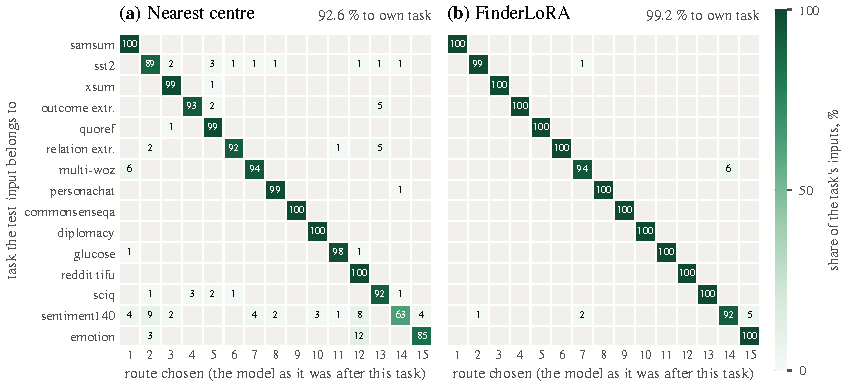
\includegraphics[width=\linewidth]{figures/route_matrix}
  \caption{Where the switch sends the test inputs: fifteen tasks without definitions, after the
  last task (seed 42). Rows: the task an input belongs to; columns: the route it gets; a cell is
  the share of the task's test inputs in per cent (shown from 1\,\%). (a)~The nearest centre sends
  \AudFifteenNoDefCentreRight{}\,\% of the inputs to their own task, (b)~\recog{}
  \AudFifteenNoDefRidgeRight{}\,\%.}
  \label{fig:routematrix}
\end{figure}


\begin{table}[t]
  \caption{The 15 SuperNI tasks without definitions, seed 42, T5-base, 10 epochs, re-test: the same plain adapters under each rule. Columns as in Table~\ref{tab:noinstfull}; the last column is the share of test inputs given to their own task after the last task. The three bottom rows are the run with definitions of Section~\ref{sec:fifteen}, for reference.}
  \label{tab:noinstfifteen}
  \centering
  {\footnotesize\setlength{\tabcolsep}{3pt}\begin{tabular}{p{1.75in}rrrrr}
    \toprule
    Method (seed 42, 15 tasks) & \shortstack[r]{Score right\\after\\learning $\uparrow$} & \shortstack[r]{Final\\score $\uparrow$} & \shortstack[r]{Forgetting\\(points) $\downarrow$} & \shortstack[r]{Answers\\changed\\of \AudFifteenNoDefCompared{} $\downarrow$} & \shortstack[r]{Sent to own\\task, \% $\uparrow$} \\
    \midrule
    \plain{} & \AudFifteenNoDefPlainLearned{} & \AudFifteenNoDefPlainAP{} & \AudFifteenNoDefPlainFT{} & \AudFifteenNoDefPlainChanged{} & \AudFifteenNoDefPlainRight{} \\
    \centre{} & \AudFifteenNoDefCentreLearned{} & \AudFifteenNoDefCentreAP{} & \AudFifteenNoDefCentreFT{} & \AudFifteenNoDefCentreChanged{} & \AudFifteenNoDefCentreRight{} \\
    \recog{} (ours) & \AudFifteenNoDefRidgeLearned{} & \AudFifteenNoDefRidgeAP{} & \AudFifteenNoDefRidgeFT{} & \AudFifteenNoDefRidgeChanged{} & \AudFifteenNoDefRidgeRight{} \\
    \handicap{} (ours) & \AudFifteenNoDefHandicapLearned{} & \AudFifteenNoDefHandicapAP{} & \AudFifteenNoDefHandicapFT{} & \AudFifteenNoDefHandicapChanged{} & \AudFifteenNoDefHandicapRight{} \\
    every input to its own task (ceiling) & \AudFifteenNoDefOwnLearned{} & \AudFifteenNoDefOwnAP{} & \AudFifteenNoDefOwnFT{} & \AudFifteenNoDefOwnChanged{} & \AudFifteenNoDefOwnRight{} \\
    \midrule
    \cert{}, with definitions & \AudFifteenDefCertLearned{} & \AudFifteenDefCertAP{} & \AudFifteenDefCertFT{} & \AudFifteenDefCertChanged{} & \AudFifteenDefCertRight{} \\
    GainLoRA, with definitions & \AudFifteenDefGainloraLearned{} & \AudFifteenDefGainloraAP{} & \AudFifteenDefGainloraFT{} & \AudFifteenDefGainloraChanged{} & -- \\
    InfLoRA, with definitions & \AudFifteenDefInfloraLearned{} & \AudFifteenDefInfloraAP{} & \AudFifteenDefInfloraFT{} & \AudFifteenDefInfloraChanged{} & -- \\
    \bottomrule
\end{tabular}}

\end{table}

\paragraph{What the results without instructions show.} This paragraph closes Sections~\ref{sec:nodefpublished}, \ref{sec:recogniser} and~\ref{sec:nodeftrained}. \emph{Reached:} without any instruction, a recogniser over all tasks that blocks nothing, stores one vector per task and one matrix for all tasks, and is the same for every order of arrival; on development data it gives \AudDevLLamOneEnd{}\% of the test inputs to their own task after 15 tasks. An audit and a bound in advance are proved (Proposition~\ref{prop:audit}, Theorem~\ref{thm:handicap}), and the measured change was within them in every run here (averages over tasks, one split each, and on the fresh batches a split that does not ensure exchangeability). Three rules passed their lines on fresh tasks, among them the \recog{} that was used on the GPU; it also passed its line on the second benchmark (\AudScaleLongThreeEnd{}\%, routes only) and still gives \AudScaleAllHundredTwentyEnd{}\% with 120 tasks. In one reduced setting, trained answers beat the two published methods that we ran without instructions, by the line fixed before (re-test against re-test). At 10 epochs most of the gap in the final score is learning; with their published \AudFullEpochs{} epochs (one seed) the two methods learn the tasks, and the gap is forgetting. The control with definitions at the same number of epochs says that the instruction is what held most of their answers (nearly all for GainLoRA, fewer for InfLoRA).
\emph{Not reached:} the published setting (a larger model; the full number of epochs was run for one seed only); the published methods on more than five tasks without definitions (ours ran on fifteen, one seed); the second benchmark with trained answers; a tight bound in advance; the published methods with an oracle for the task, or with our recogniser in front of them; the upper side of the conflict $\Omega$ (the error of the best classifier between two tasks); and inputs that occur in two tasks, which no method without instructions can do better than split.
Choices made after seeing numbers (the features, \handicap{} and its floor, the zone shapes) give development numbers; only the fresh batches and the GPU run were read once against lines written before.
